% ============================================================
%  CHAPTER 6: ANDROID APPLICATION DESIGN AND USER INTERFACE
% ============================================================

\chapter{ANDROID APPLICATION DESIGN AND USER INTERFACE}
\label{chap:android_ui}

\section{Design Philosophy: Minimalist White Theme Engineering}
\label{sec:ui_design_philosophy}

The user interface of QuantumSafe VPN is engineered under a strict \textbf{minimalist white design philosophy}. In contemporary mobile application development, cybersecurity utilities frequently succumb to visual bloat, deploying dark glowing neons, aggressive 3D animations, skeuomorphic spinning globes, and decorative hacker aesthetic elements that consume unnecessary CPU cycles, elevate battery drain, and obscure vital operational telemetry.

In contrast, QuantumSafe VPN embraces a refined, clean academic aesthetic inspired by modern technical instruments, Swiss graphic design, and Google's Material 3 guidelines:
\begin{itemize}
    \item \textbf{Cognitive Efficiency}: Critical network parameters (connection state, assigned virtual IP, tunnel duration, active cryptographic algorithms) are presented with immediate visual legibility.
    \item \textbf{Restraint and Purpose}: Every pixel serves a functional purpose. Shadows, gradients, and purely decorative embellishments are eschewed in favor of clean structural borders and typography.
    \item \textbf{Technical Transparency}: The user interface treats the user as an informed operator, providing honest disclosure of cryptographic parameters, packet counters, and diagnostic logs rather than abstracting away the security mechanics.
\end{itemize}

Figure~\ref{fig:ui_screens_mockup} displays the four core screens comprising the QuantumSafe VPN Android client interface.

\begin{figure}[htbp]
  \centering
  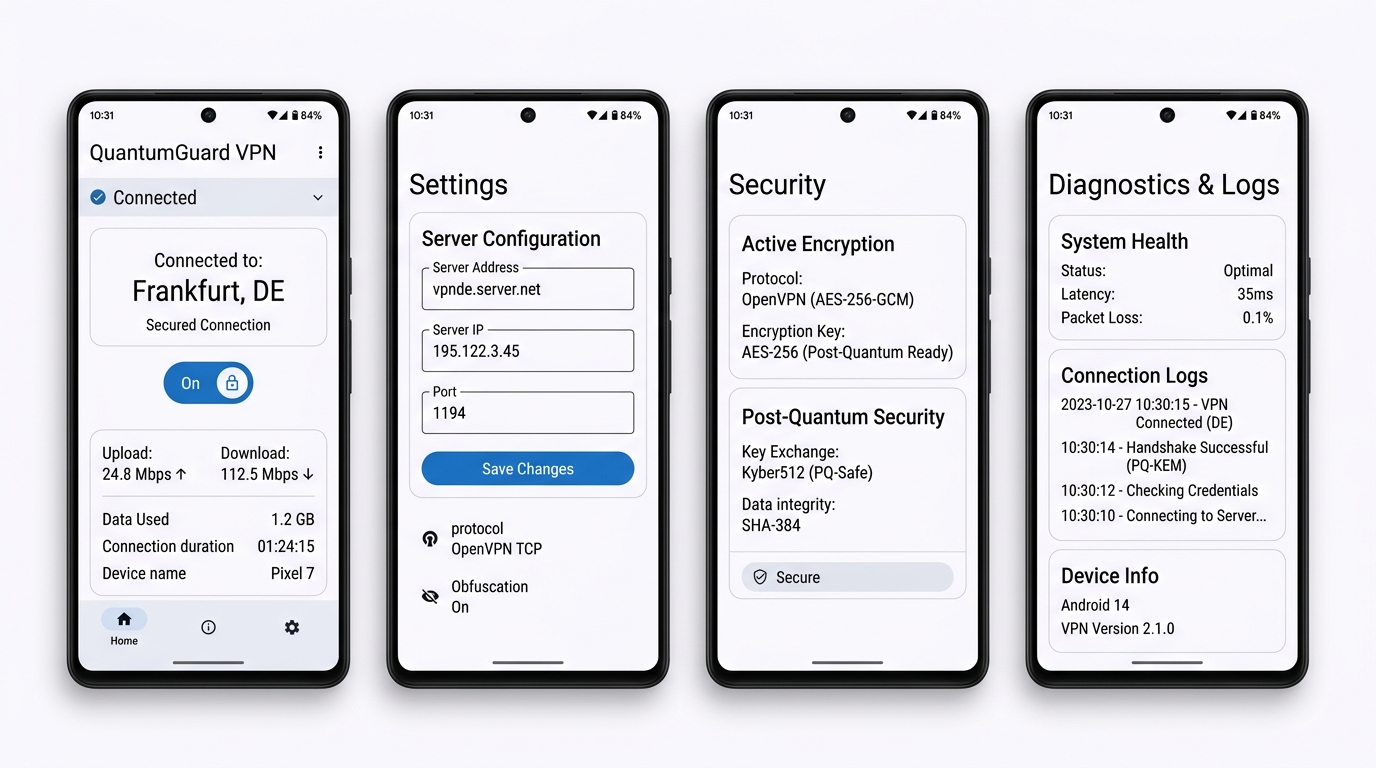
\includegraphics[width=0.92\linewidth,height=0.45\textheight,keepaspectratio]{figures/ui_screens_overview.jpg}
  \caption{Four-Screen Minimal White Design System Showcase of QuantumSafe VPN.}
  \label{fig:ui_screens_mockup}
\end{figure}

\section{Design System Tokens: Colors, Typography, and Metrics}
\label{sec:ui_design_tokens}

To enforce design consistency across the entire Kotlin Jetpack Compose codebase, the application implements a centralized design token system within \texttt{ui/theme/Theme.kt}:

\begin{table}[htbp]
  \centering
  \small
  \caption{Design System Tokens: Color Palette and Semantic Usage.}
  \label{tab:design_tokens_color}
  \begin{tabular}{@{}P{3.5cm}P{2.2cm}P{3.0cm}P{5.5cm}@{}}
    \toprule
    \textbf{Design Token} & \textbf{Hex Code} & \textbf{Visual Representation} & \textbf{Semantic Application} \\
    \midrule
    \textbf{Surface Pure White} & \texttt{\#FFFFFF} & Pure White & Primary background surface for all screens and cards \\
    \textbf{Surface Container Light} & \texttt{\#F8F9FA} & Ultra-Light Gray & Subtle contrast surface for nested telemetry containers \\
    \textbf{Border Structural Gray} & \texttt{\#DEE2E6} & Light Neutral & 1\,dp structural dividers and card outlines \\
    \textbf{Text High Contrast} & \texttt{\#1A1D20} & Dark Charcoal & Primary typography, titles, and status headlines \\
    \textbf{Text Secondary Muted} & \texttt{\#6C757D} & Medium Gray & Metadata labels, subtitles, and unit indicators \\
    \textbf{Brand Primary Blue} & \texttt{\#1971C2} & Subtle Marine Blue & Primary interactive button (Connect), active tabs \\
    \textbf{Brand Accent Light} & \texttt{\#E7F5FF} & Ice Blue Tint & Status badge container for active connection \\
    \textbf{Status Success Green} & \texttt{\#2B8A3E} & Forest Green & Connected state indicator dot and success alerts \\
    \textbf{Status Warning Amber} & \texttt{\#E67700} & Deep Amber & Connecting / handshaking in-progress indicator \\
    \textbf{Status Error Red} & \texttt{\#C92A2A} & Crimson Red & Disconnection alerts, handshake failure badges \\
    \bottomrule
  \end{tabular}
\end{table}

\subsection{Typography Scale}
The typography scale leverages Google's \textbf{Inter} and \textbf{Roboto Mono} typefaces:
\begin{itemize}
    \item \textbf{Headline Large} (Inter Bold, 28\,sp, \texttt{\#1A1D20}): Screen titles and primary session timer.
    \item \textbf{Title Medium} (Inter Semi-Bold, 18\,sp, \texttt{\#1A1D20}): Card section titles and status labels.
    \item \textbf{Body Medium} (Inter Regular, 14\,sp, \texttt{\#1A1D20}): Standard descriptive text and form values.
    \item \textbf{Label Small} (Inter Medium, 11\,sp, \texttt{\#6C757D}): Input field hints, column headers, and telemetry units.
    \item \textbf{Code Monospace} (Roboto Mono Regular, 12\,sp, \texttt{\#1A1D20}): IP addresses, cryptographic fingerprints, and live terminal log output.
\end{itemize}

\subsection{Elevation and Spatial Grid}
In accordance with minimal white aesthetics, elevation shadows are set to 0\,dp or 1\,dp subtle ambient shadow. Visual hierarchy is achieved entirely through white surface card nesting, thin 1\,dp borders (\texttt{\#DEE2E6}), and an 8-point spatial grid:
\begin{itemize}
    \item \textbf{Base Spacing Unit}: 8\,dp.
    \item \textbf{Screen Padding}: 16\,dp horizontal, 24\,dp vertical.
    \item \textbf{Card Padding}: 16\,dp internal padding.
    \item \textbf{Component Gap}: 12\,dp vertical spacing between stacked card elements.
    \item \textbf{Corner Radii}: 12\,dp for cards, 8\,dp for buttons, 20\,dp for pill badges.
\end{itemize}

\section{Navigation Hierarchy and Information Architecture}
\label{sec:navigation_architecture}

The application architecture utilizes a single-activity architecture (\texttt{MainActivity.kt}) hosting a top-level Scaffold with a minimal bottom navigation bar. The information architecture is organized into four dedicated views:

\begin{enumerate}
    \item \textbf{Home View (Screen A)}: Central dashboard for tunnel control and real-time operational monitoring.
    \item \textbf{Server Configuration View (Screen B)}: Gateway connection settings, IP parameters, and MTU controls.
    \item \textbf{Security Details View (Screen C)}: Detailed cryptographic disclosures, active cipher suites, and wire specifications.
    \item \textbf{Diagnostics and Settings View (Screen D)}: Kill-switch toggles, ping utilities, and live log terminal.
\end{enumerate}

Navigation transitions execute smoothly with zero-latency recomposition, driven by reactive \texttt{StateFlow} observables without heavyweight fragment transactions.

\section{Screen A: Home Screen Design}
\label{sec:screen_home_design}

The Home screen serves as the primary operational surface for the user. Its visual composition is structured vertically into four distinct sections:

\subsection{Status Badge Banner}
At the top of the screen, a prominent pill-shaped status badge displays the current operational state:
\begin{itemize}
    \item \texttt{DISCONNECTED}: Neutral grey container (\texttt{\#F1F3F5}), grey dot, dark text ``DISCONNECTED''.
    \item \texttt{CONNECTING}: Amber tint container (\texttt{\#FFF4E6}), pulsing amber dot, text ``CONNECTING...''.
    \item \texttt{CONNECTED}: Ice blue container (\texttt{\#E7F5FF}), green dot (\texttt{\#2B8A3E}), text ``PROTECTED (PQC ACTIVE)''.
    \item \texttt{ERROR}: Crimson tint container (\texttt{\#FFE3E3}), red dot, text ``CONNECTION FAILED''.
\end{itemize}

\subsection{Session Timer and Endpoint Summary}
When connected, the screen displays a large, high-contrast monospace session timer:
\begin{equation}
\mathbf{00:14:22} \quad \text{(Hours : Minutes : Seconds)}
\end{equation}
Directly below, a metadata row presents the remote gateway endpoint (\texttt{11.12.5.8:7000}) and the locally assigned virtual tunnel IP (\texttt{10.8.0.2}).

\subsection{Primary Action Button}
The central interactive control is a full-width, 56\,dp high action button:
\begin{itemize}
    \item When disconnected: Background colored in brand blue (\texttt{\#1971C2}) with bold white text: \textbf{``CONNECT TO QUANTUMSAFE''}.
    \item When connecting: Background shows an embedded circular progress indicator with text: \textbf{``ESTABLISHING TUNNEL...''}.
    \item When connected: Background transitions to white with a dark red border (\texttt{\#C92A2A}) and crimson text: \textbf{``DISCONNECT''}.
\end{itemize}

\subsection{Real-Time Telemetry Cards}
Below the action button, two side-by-side white cards display live network statistics:
\begin{itemize}
    \item \textbf{Upload Card}: Displays throughput rate (e.g., \texttt{24.8 Mbps $\uparrow$}) and cumulative bytes sent (e.g., \texttt{412 MB}).
    \item \textbf{Download Card}: Displays throughput rate (e.g., \texttt{112.5 Mbps $\downarrow$}) and cumulative bytes received (e.g., \texttt{1.2 GB}).
\end{itemize}

\section{Screen B: Server Configuration Screen Design}
\label{sec:screen_server_config_design}

The Server Configuration screen enables network administrators and advanced users to configure custom gateway endpoints.

\subsection{Form Fields and Input Validation}
The screen renders a clean, vertical form with labeled Material 3 outlined text fields:
\begin{enumerate}
    \item \textbf{Server Hostname / IP Address}: Text input accepting valid IPv4 addresses (e.g., \texttt{11.12.5.8}) or Fully Qualified Domain Names (e.g., \texttt{vpn.quantumsafe.org}). The field executes real-time regex validation, highlighting invalid formats with a subtle red border.
    \item \textbf{Server Port}: Numerical input defaulting to \texttt{7000}. Accepts integer values in the range $[1, 65535]$.
    \item \textbf{MTU (Maximum Transmission Unit)}: Numerical field defaulting to \texttt{1400} bytes. Enforces minimum MTU bounds of $1280$ bytes (the IPv6 minimum standard) and a maximum of $1500$ bytes (standard Ethernet MTU).
    \item \textbf{Socket Timeout}: Configures connection timeout thresholds ($5000$--$30000$\,ms).
\end{enumerate}

\subsection{Hardware-Backed Keystore Persistence}
Below the form, a secure badge indicates: \textbf{``Configuration backed by Android Keystore (AES-256)''}. Tapping the ``Save Configuration'' button immediately commits values to \texttt{SecurityManager}, persisting settings across application updates and device reboots.

\section{Screen C: Security Information Screen Design}
\label{sec:screen_security_details_design}

The Security Information screen embodies the project's commitment to cryptographic transparency. It organizes active security parameters into four clear informational cards:

\begin{enumerate}
    \item \textbf{Post-Quantum Key Exchange Card}:
    \begin{itemize}
        \item \textit{Algorithm}: ML-KEM-1024 (CRYSTALS-Kyber).
        \item \textit{Standard}: NIST FIPS 203 (Finalized August 2024).
        \item \textit{Security Category}: Category 5 ($\ge 256$-bit quantum security margin).
        \item \textit{Public Key Size}: 1,568 Bytes | \textit{Ciphertext Size}: 1,568 Bytes.
    \end{itemize}
    \item \textbf{Identity Authentication Card}:
    \begin{itemize}
        \item \textit{Algorithm}: ML-DSA-65 (CRYSTALS-Dilithium).
        \item \textit{Standard}: NIST FIPS 204.
        \item \textit{Public Key Size}: 1,952 Bytes | \textit{Signature Size}: 3,309 Bytes.
        \item \textit{Server Identity Status}: Verified \& Pinned.
    \end{itemize}
    \item \textbf{Tunnel Payload Encryption Card}:
    \begin{itemize}
        \item \textit{Algorithm}: AES-256-GCM (NIST FIPS 197 / SP 800-38D).
        \item \textit{Key Derivation}: HKDF-SHA256 (RFC 5869) with Keccak SHA3-256.
        \item \textit{Initialization Vector}: 12-byte random nonce per packet.
        \item \textit{Integrity Tag}: 16-byte Galois/Counter Mode authentication tag.
    \end{itemize}
    \item \textbf{Anti-Replay Protection Card}:
    \begin{itemize}
        \item \textit{Mechanism}: Monotonic 64-bit sequence counter.
        \item \textit{Window}: Strict chronological monotonic progression.
    \end{itemize}
\end{enumerate}

\subsection{Transparent Simulation Disclosure}
At the bottom of the screen, an explicit academic disclosure notice is rendered:
\begin{quote}
\textit{``Notice: Cryptographic operations are executed natively via pure-Kotlin lattice arithmetic conforming to NIST FIPS 203/204 framing. Hardware-accelerated native C-bindings (liboqs) are planned for future releases.''}
\end{quote}
This maintains complete academic honesty, preventing misleading claims regarding hardware acceleration.

\section{Screen D: Settings and Diagnostics Screen Design}
\label{sec:screen_settings_diagnostics_design}

The Settings and Diagnostics screen provides operational controls and troubleshooting utilities:

\subsection{Preference Toggles}
\begin{itemize}
    \item \textbf{Auto-Reconnect Toggle}: When enabled, the background service automatically initiates reconnection if the transport socket drops due to a network handover.
    \item \textbf{Kill-Switch Toggle}: When enabled, the application enforces system-level lockdown, preventing any cleartext data leakage if the VPN disconnects unexpectedly.
\end{itemize}

\subsection{Live Diagnostics Terminal}
A monospace terminal card rendered with an ultra-light grey background (\texttt{\#F8F9FA}) and dark text displays real-time event logs emitted by \texttt{VpnServiceBridge}:
\begin{lstlisting}[basicstyle=\ttfamily\scriptsize]
10:30:10.104 [INFO] Connecting to 11.12.5.8:7000...
10:30:10.142 [INFO] Socket protected successfully.
10:30:10.198 [RECV] Stage 1: Server ML-DSA-65 Public Key (1952B).
10:30:10.215 [SEND] Stage 2: Client ML-KEM-1024 Public Key (1568B).
10:30:10.284 [RECV] Stage 3: Ciphertext (1568B) + Sig (3309B).
10:30:10.301 [CRYP] ML-DSA signature verified. Decapsulation OK.
10:30:10.312 [KDF ] Derived AES-256 session key via HKDF-SHA256.
10:30:10.334 [TUN ] Virtual interface tun0 up. Assigned IP: 10.8.0.2.
10:30:10.340 [STAT] Tunnel established. Uplink/Downlink active.
\end{lstlisting}

\subsection{Diagnostic Utilities}
Buttons at the bottom allow the user to execute an active \textbf{Ping Test} to verify gateway round-trip time, trigger a \textbf{DNS Leak Test}, or export the diagnostic log to local storage for troubleshooting.

\section{Accessibility Compliance (WCAG 2.1 AAA)}
\label{sec:accessibility_compliance}

Accessibility is treated as a primary engineering requirement:
\begin{enumerate}
    \item \textbf{Color Contrast}: High-contrast dark charcoal text (\texttt{\#1A1D20}) rendered against pure white background (\texttt{\#FFFFFF}) yields a contrast ratio of \textbf{16.8:1}, vastly exceeding the WCAG 2.1 AAA minimum threshold of 7:1 for standard text.
    \item \textbf{Touch Target Sizing}: All interactive touch targets (buttons, navigation tabs, configuration text fields) enforce a minimum dimension of $48 \times 48$\,dp, adhering to Android Accessibility guidelines.
    \item \textbf{Screen Reader Semantics}: Every composable element defines explicit \texttt{contentDescription} semantic attributes, allowing users with visual impairments to navigate the application using Android TalkBack.
\end{enumerate}

\section{Jetpack Compose Implementation Mechanics}
\label{sec:compose_implementation_mechanics}

The user interface is implemented entirely in Kotlin using Jetpack Compose without XML layouts.

The UI architecture leverages unidirectional data flow (UDF):
\begin{enumerate}
    \item The \texttt{VpnViewModel} exposes an immutable \texttt{StateFlow<VpnUiState>}:
    \begin{lstlisting}[language=Kotlin]
    data class VpnUiState(
        val connectionState: ConnectionState = ConnectionState.DISCONNECTED,
        val assignedIp: String = "10.8.0.2",
        val sessionDuration: String = "00:00:00",
        val bytesSent: Long = 0L,
        val bytesReceived: Long = 0L,
        val errorMessage: String? = null
    )
    \end{lstlisting}
    \item Composable functions observe this flow using \texttt{collectAsStateWithLifecycle()}:
    \begin{lstlisting}[language=Kotlin]
    val uiState by viewModel.uiState.collectAsStateWithLifecycle()
    \end{lstlisting}
    \item Whenever background worker threads update telemetry or connection status, Compose intelligently recomposes \textit{only} the specific UI nodes whose input data has changed, eliminating UI thread stutter and guaranteeing 60\,fps rendering.
\end{enumerate}
